\begin{figure}[H]
\centering
	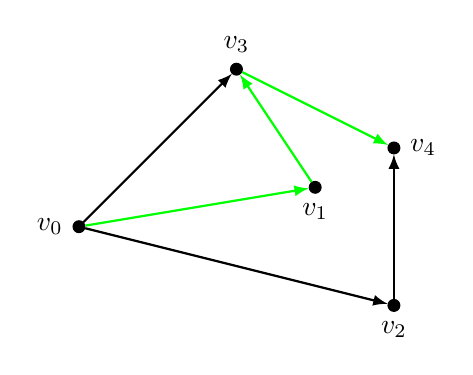
\begin{tikzpicture}

      \tikzset{enclosed/.style={draw, circle, inner sep=0pt, minimum size=.15cm, fill=black}}
%% Vertices
      	\node[enclosed, label={left: $v_0$}] (v0) at (0,2) {};
      	\node[enclosed, label={below: $v_1$}] (v1) at (3,2.5) {};
    		\node[enclosed, label={below: $v_2$}] (v2) at (4,1) {};
  	    \node[enclosed, label={above: $v_3$}] (v3) at (2,4) {};
     	\node[enclosed, label={right: $v_4$}] (v4) at (4,3) {};
%Edges
		\path [->, >=latex, thick, green](v0) edge node[midway, sloped, above] {} (v1);
		\path [->, >=latex, thick](v0) edge node[midway, sloped, above] {} (v2);
		\path [->, >=latex, thick](v0) edge node[midway, above] {} (v3);
		\path [->, >=latex, thick, green](v1) edge node[near end, sloped, below] {} (v3);
		\path [->, >=latex, thick](v2) edge node[midway, below] {} (v4);
		\path [->, >=latex, thick, green](v3) edge node[near end, sloped, above] {} (v4);

	\end{tikzpicture}
	\caption{Eksempel på en orienteret simpel graf og en vej fra $v_{0}$ til $v_{4}$}
	\label{fig.vaegtetopg}
\end{figure}